%TCIDATA{LaTeXparent=0,0,RUL1.tex}

\begin{biography}[{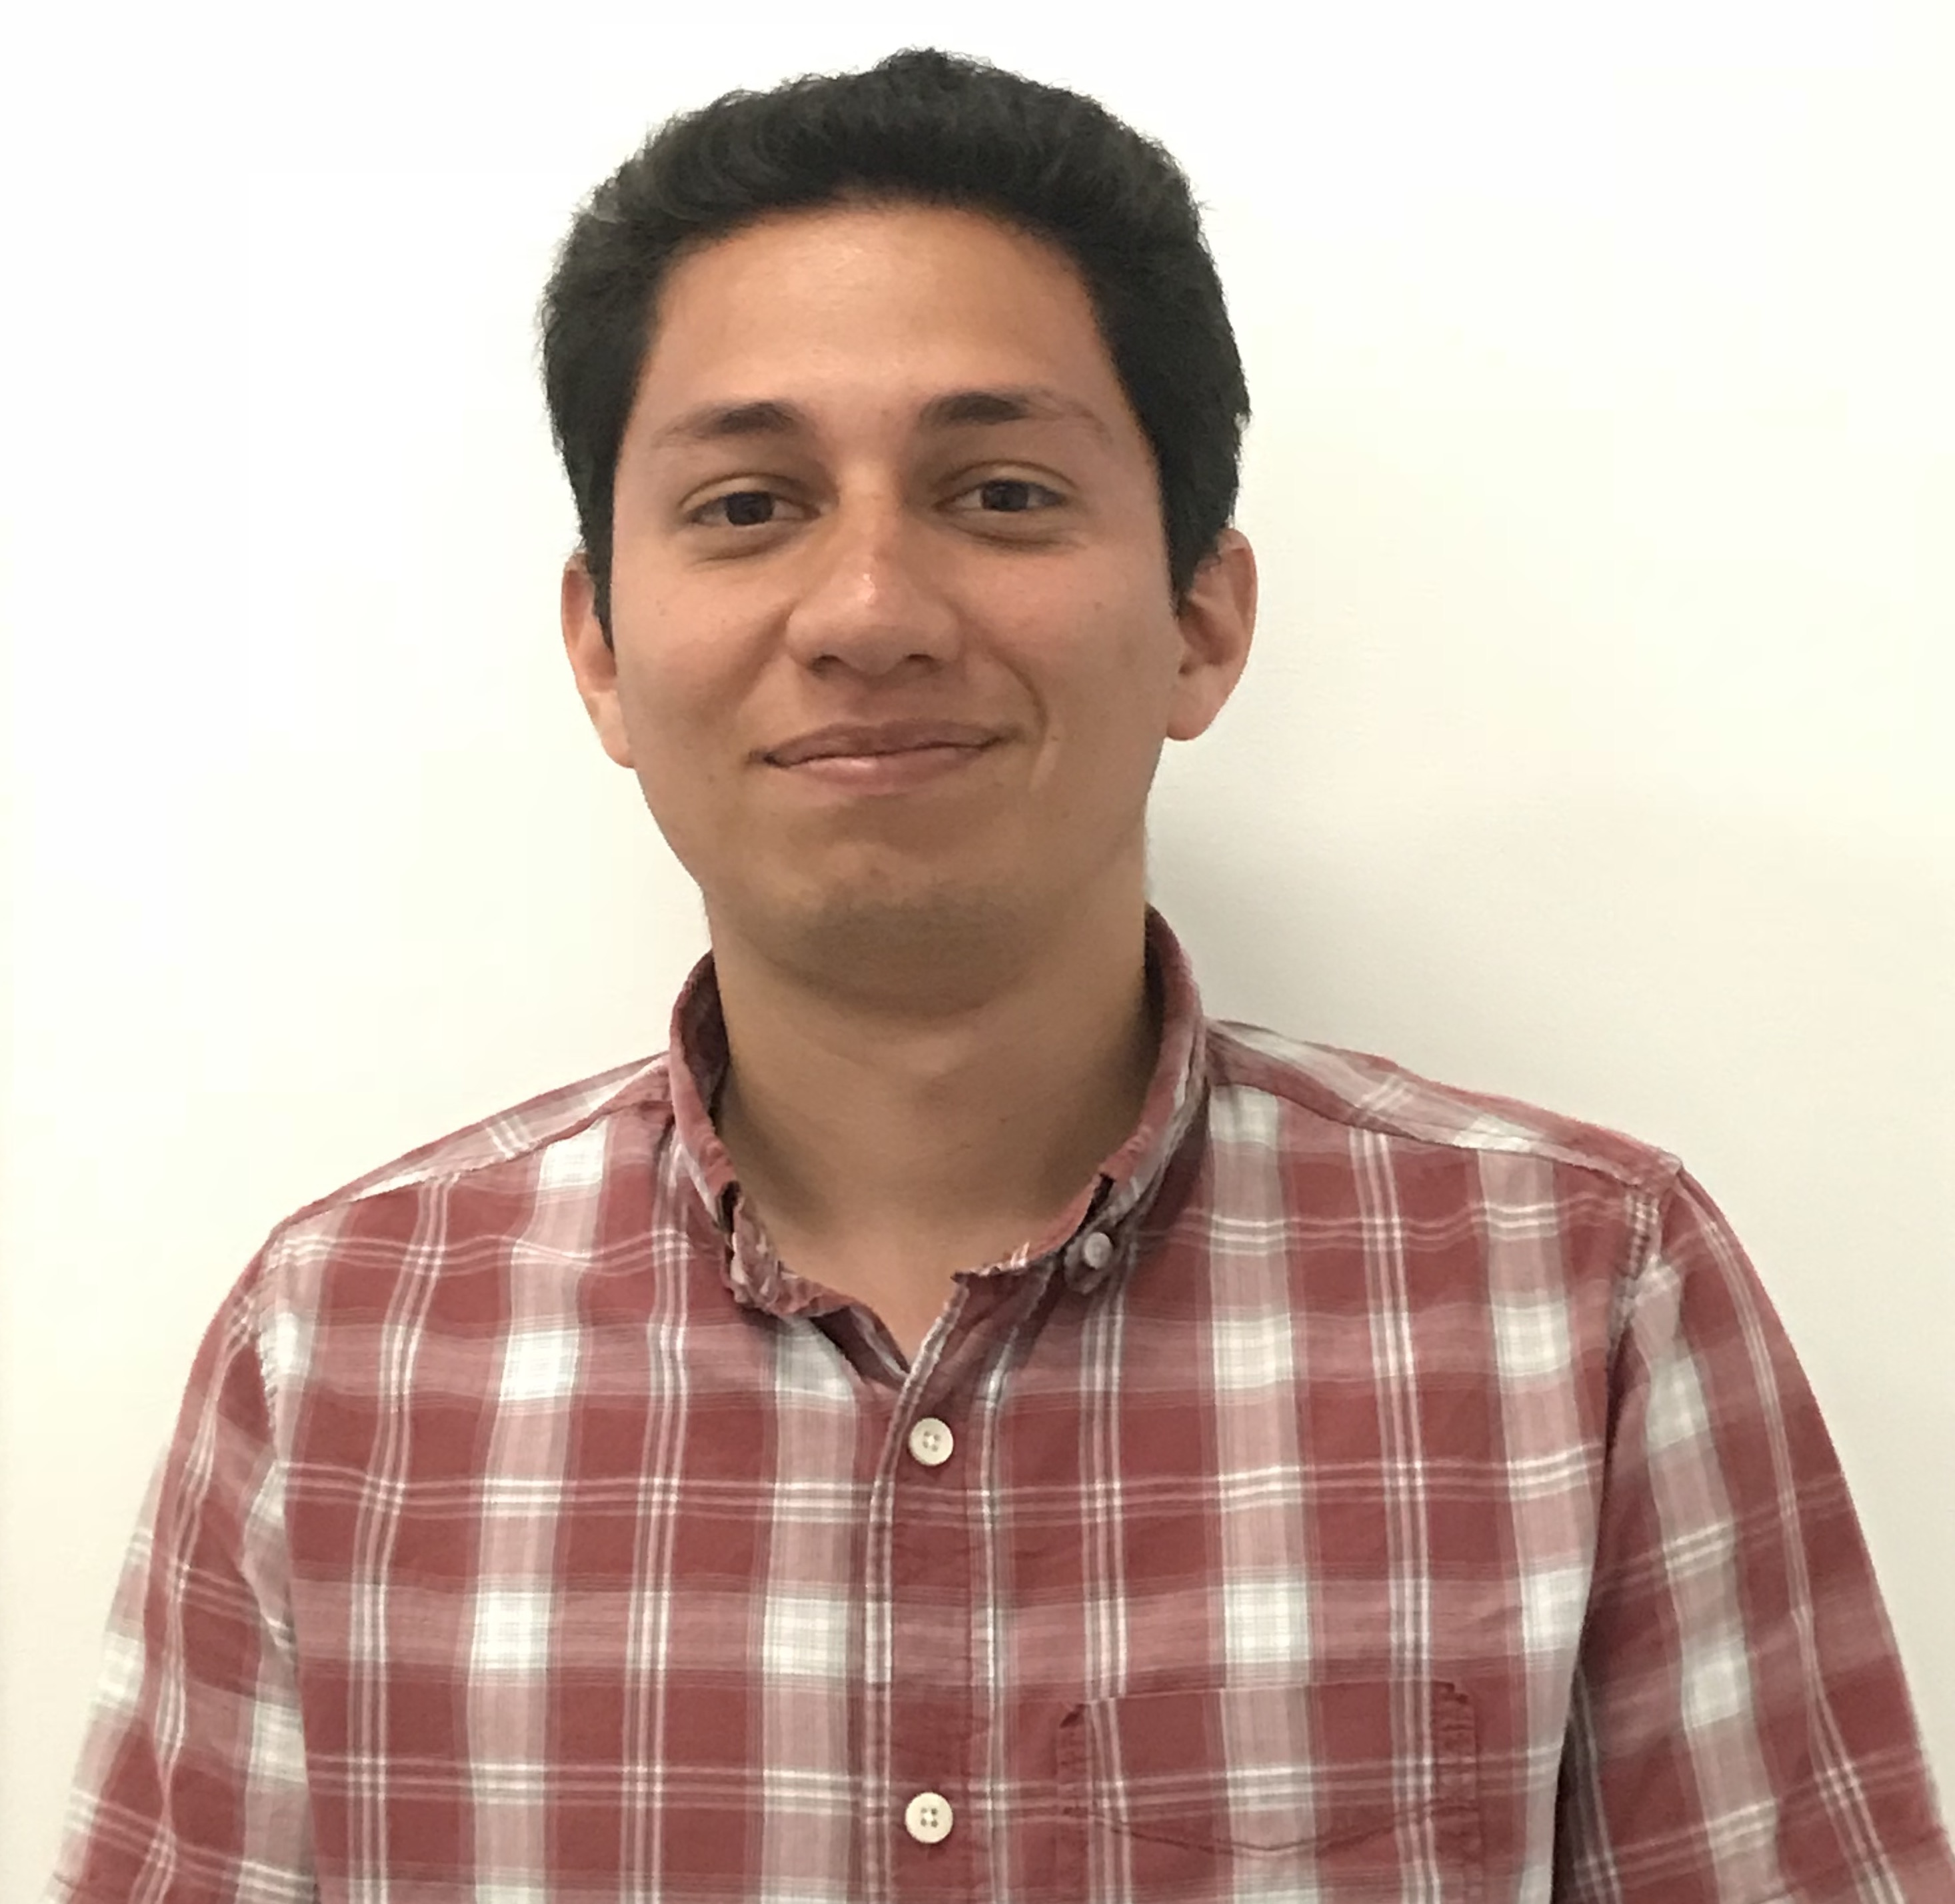
\includegraphics[width=1in,height=1.25in, clip]{BioPhotos/dlr.jpg}}]{David Laredo}
is a Masters student in Mechanical Engineering at the UC Merced under the supervision of Dr. Jian-Qiao Sun since 2016. He earned a BS degree in Computer Science from ESCOM-IPN in 2012 and a Masters in Computer Science from CINVESTAV-IPN in 2015. His research interest are numerical optimization, machine learning methods for engineering problems, machine learning model selection and hyper-parameter tuning.
\end{biography}

\begin{biography}[{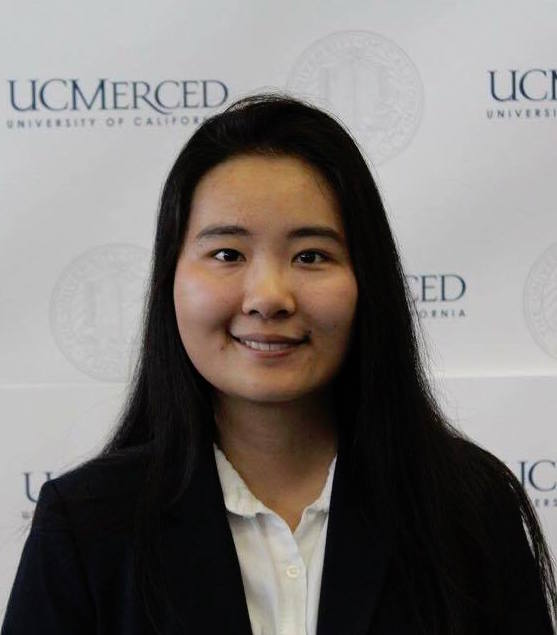
\includegraphics[width=1in,height=1.25in,clip]{BioPhotos/ZhaoyinChen.jpg}}]{Zhaoyin Chen}
is an undergraduate student in Computer Science and Engineering at the University of California,
Merced. For over a year, she has worked in the Applied Controls
Lab led by Dr. Jian-Qiao Sun, where she applies deep learning to her research.
She is interested in database, model training and finding the most
suitable architecture for each problem. She is involved
with the Association for Computing Machinery and serves
on the leadership board as the treasurer. She is a multiple time
recipient of the Chancellor?s Honor List award.
\end{biography}

\begin{biography}[{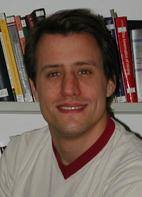
\includegraphics[width=1in,height=1.25in,clip]{BioPhotos/ols.jpg}}]{Oliver Sch\"utze}
received the Diploma degree in mathematics from the University
of Bayreuth, Bayreuth, Germany, and the Ph.D. degree in natural
sciences from the University of Paderborn, Paderborn, Germany, in
1999 and 2004, respectively. He is
currently a Professor (CINVESTAV-3A Re-searcher) with the Department
of Computer Science, CINVESTAV-IPN, Mexico City, Mexico. He serves as Editor-in-Chief of Mathematical and Computational Applications by MDPI. His research interests include the design and analysis of numerical and evolutionary optimization algorithms.
\end{biography}

\begin{biography}[{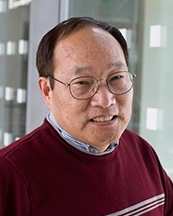
\includegraphics[width=1in,height=1.25in,clip]{BioPhotos/jqs.jpg}}]{Jian-Qiao Sun}
earned a BS degree in Solid Mechanics from Huazhong University of Science and Technology in 1982, and PhD in Mechanical Engineering from University of California at Berkeley in 1988.  In 1994, Dr. Sun joined the faculty of the department of Mechanical Engineering at the University of Delaware as an Assistant Professor, was promoted to Associate Professor in 1998 and to Professor in 2003.  Dr. Sun joined the new campus of University of California at Merced in 2007 and is currently Professor and Chair of Mechanical Engineering. He serves as the Editor-in-Chief of the International Journal of Dynamics and Control by Springer.  His research interests include random vibrations, nonlinear controls, energy harvesting technologies, and data-driven modeling and analysis of complex mechanical systems.
\end{biography}


